\documentclass[my_thesis.tex]{subfiles}

\begin{document}
\cleardoublepage
\chapter*{Introduction}
\markboth{Introduction}{Introduction}
\addcontentsline{toc}{chapter}{Introduction}

\section{The need for new sources of energy}



\section{Nuclear fusion as a source of energy}
Nuclear fusion is the process of forming a nucleus from two, lighter nuclei. This, in particular, is the process that powers all stars in the universe. Nuclear \emph{fusion} is the opposite of nuclear \emph{fission}, where two nuclei are formed by breaking one, heavier nucleus. Nuclear fission is commonly used to power nuclear fission power plants.

Atomic nuclei are composed of neutron and protons, and are kept bound together by the strong interaction. The binding energy of the nucleon, defined as the minimum energy required to separate a nucleus as a collection of its nucleon, measures then how tightly bound a nucleus is. The binding energy per nucleon, shown on Figure \ref{fig. binding energy}, is low for hydrogen, grows with atomic number until reaching a maximum for the iron, and then decreases with increasing atomic number. Fusing two nuclei lighter than iron will then, in general, release energy.

\begin{figure}
    \centering
    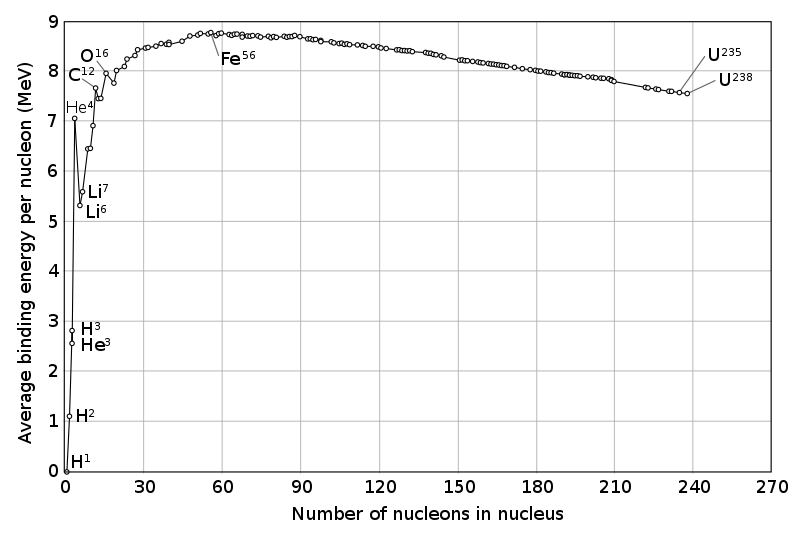
\includegraphics[width=.75\linewidth]{images/introduction/BindingEnergy.png}
    \caption{Binding energy per nucleon.}
    \label{fig. binding energy}
\end{figure}

Of particular interest for commercial fusion power plants is the fusion of deuterium $\ce{H2}$ with tritium $\ce{H3}$, which generates a nucleus of helium $\ce{He4}$ with $3.5$MeV of kinetic energy, and a neutron with $14.1$MeV of kinetic energy (see Figure \ref{fig. dt fusion}). Among potential fusion reactions, this is the most promising, because the reaction cross-section is the highest. Nevertheless, deuterium-tritium fusion reactions require a temperate of at least $10$keV, \textit{i.e.} 100 millions degrees. 
\begin{figure}
    \centering
    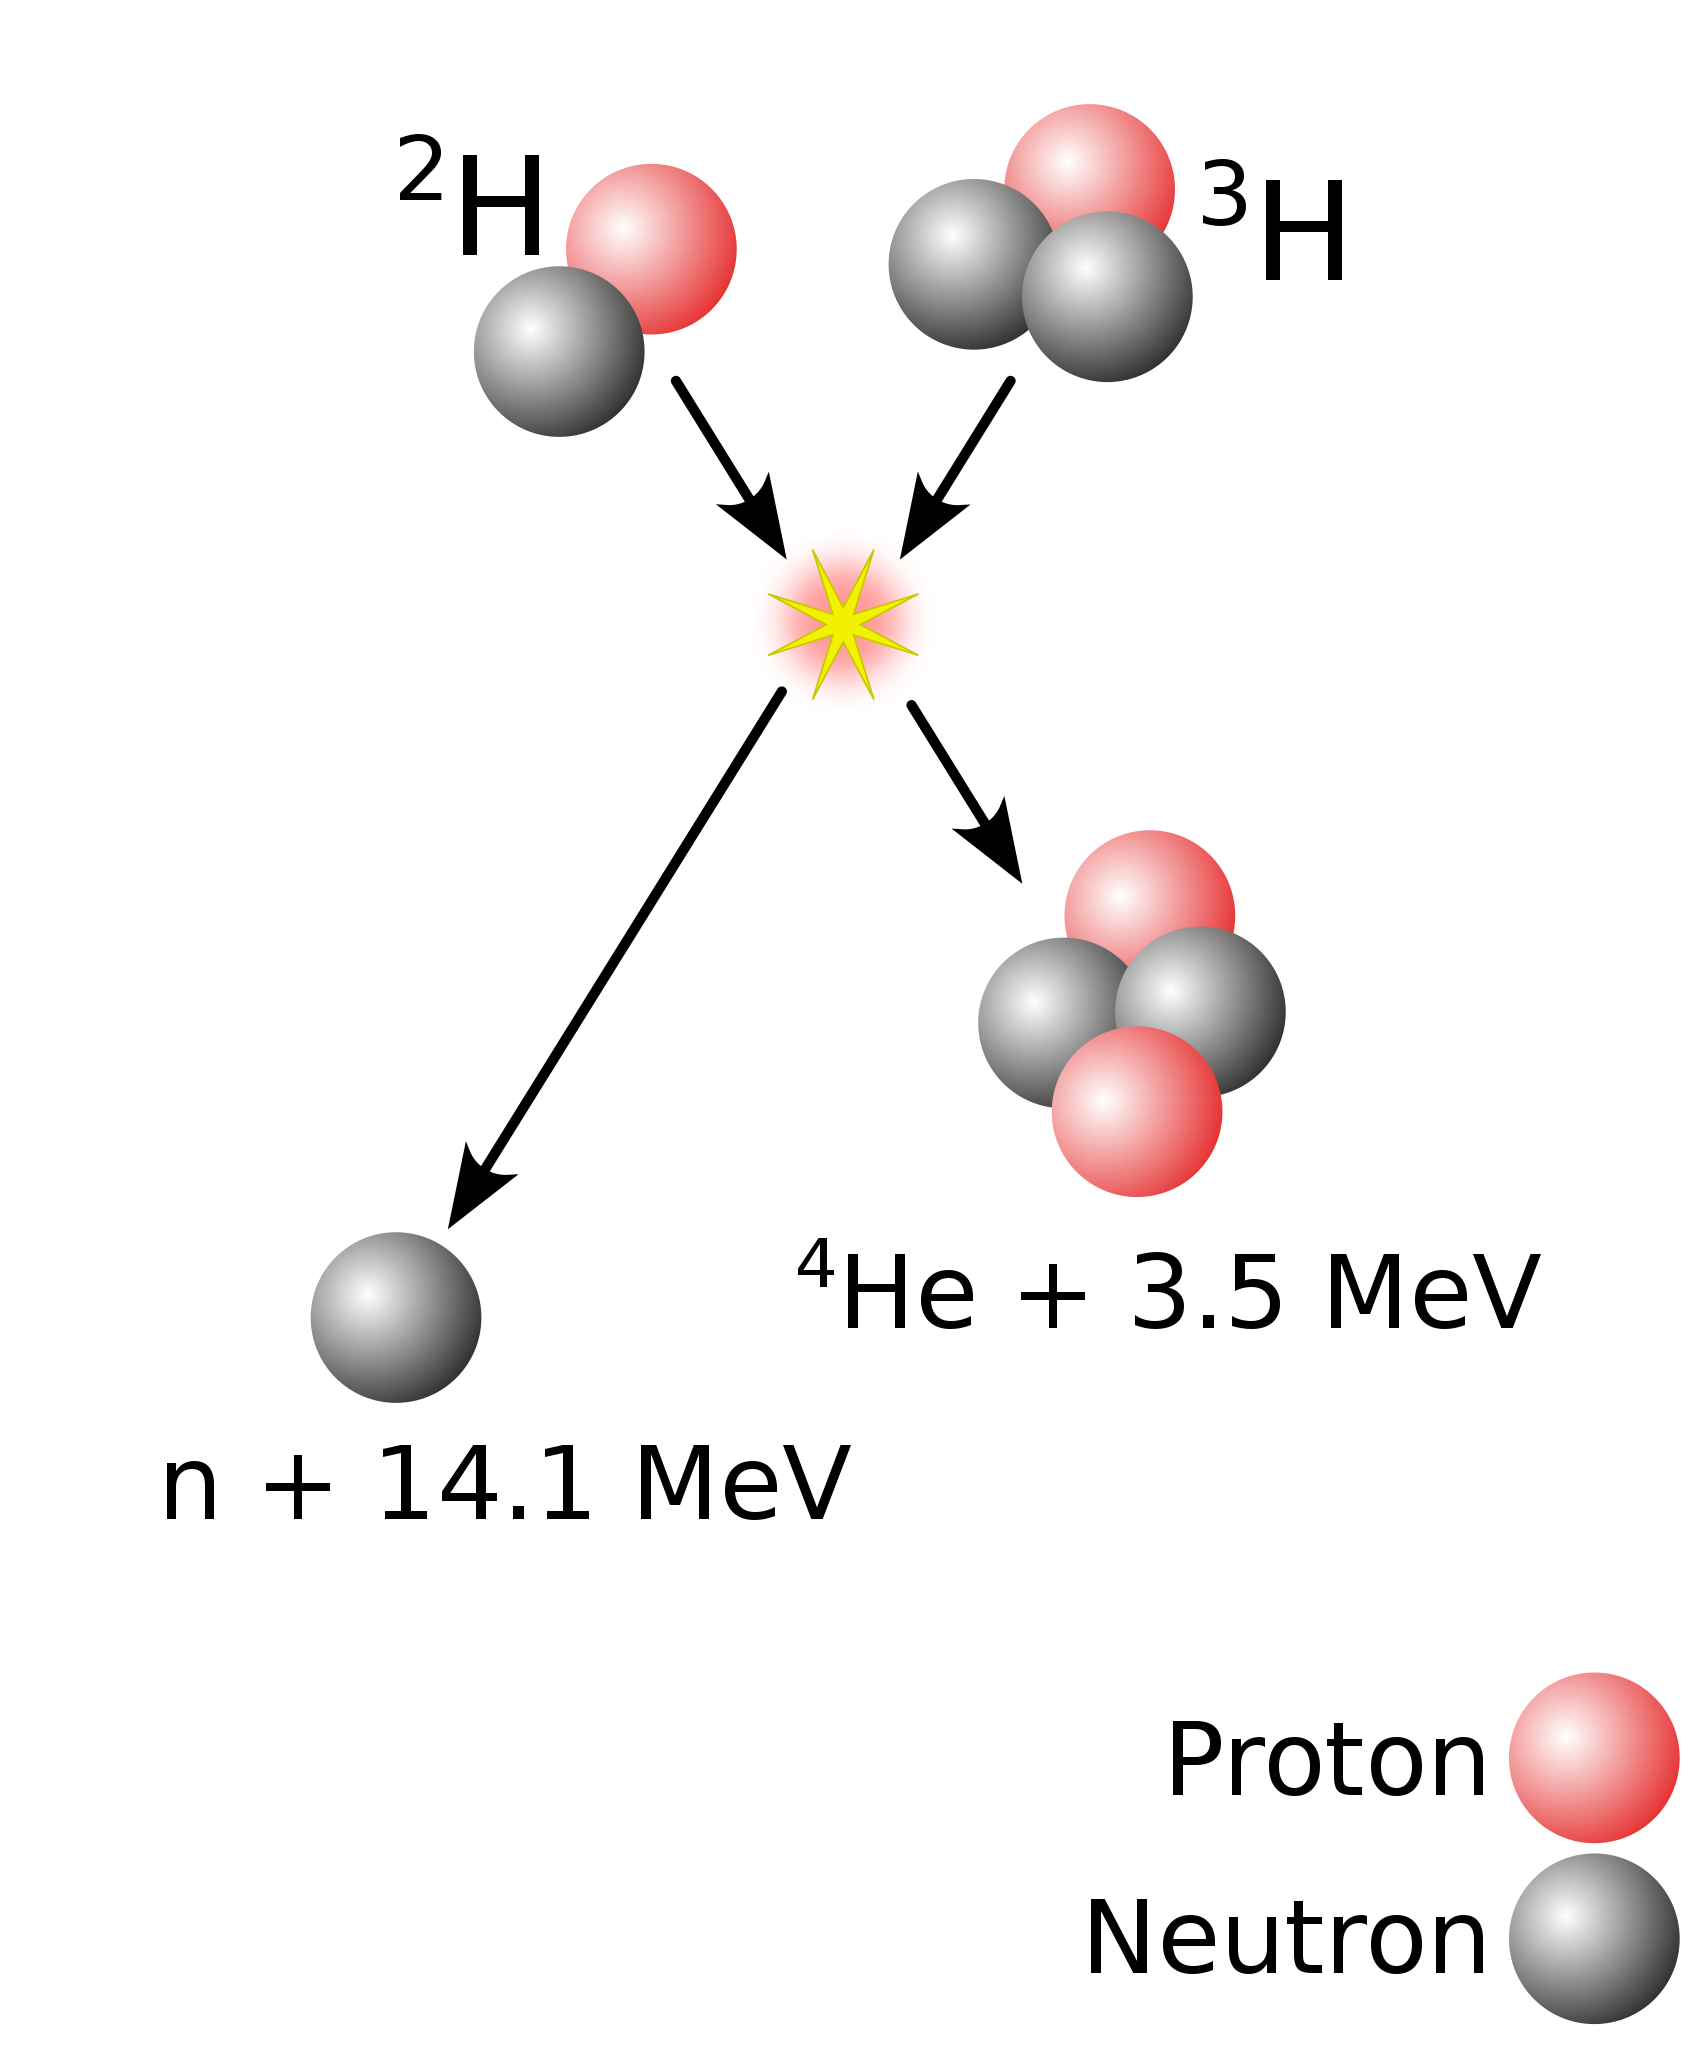
\includegraphics[width=.5\linewidth]{images/introduction/DTFusion.png}
    \caption{Sketch of a Deuterium-Tritium fusion reaction.}
    \label{fig. dt fusion}
\end{figure}

The challenge is then to confine the fuel, which forms a plasma at these temperature, for a sufficient time such that enough reactions have the time to occur. More specifically, to get energy break-even (\textit{i.e.} to get as much fusion power as input power, $Q=F_{fus}/P_{in}=1$), one can derive the so-called Lawson criterion \citep{lawsonCriteriaPowerProducing1957}, which gives a criterion on the fusion triple product,
\begin{equation}
    nT\tau_E > 1.5\cdot 10^{21}\text{keV s m}^{-3}, 
\end{equation} 
where $n$ is the plasma density, $T$ is its temperature, and $\tau_E$ is the energy confinement time. In addition, the plasma temperature cannot be too low nor too large, otherwise Bremsstrahlung losses would be too large. From this simple criterion, one can identify two paths toward a nuclear fusion power plant: (i) inertial fusion, where one maximizes the density for a very short amount of time, or (ii) magnetic confinement, where one keeps comparatively lower densities, but increases as much as possible the energy confinement time. This thesis will focus on one particular design of magnetic confinement reactor called the stellarator, which we explain in the next section.


\subsection{The stellarator concept}
The stellarator is a magnetic confinement device concept, that has the shape of a torus. In what follows, we will define the toroidal direction as the long way around the torus, and the poloidal direction as the short way around it. It can be shown that single particle confinement can not be obtained by a purely toroidal magnetic field. The particle will drift and quickly exit the plasma. 

Instead, one has to design a magnetic field that has both a toroidal and a poloidal component, which makes magnetic field lines wrap around the torus. This twist of the magnetic field line is measured by the rotational transform $\iotabar$, and can be generated by three mechanisms \citep{Helander2014}: (i) driving a toroidal current in the plasma, or (ii) shaping the plasma as a rotating ellipse close to the axis, or (iii) having magnetic axis torsion.

The tokamak, an other magnetic fusion device concept, uses only the first possibility. A strong toroidal current is driven in the plasma by an external transformer, and this produces the poloidal magnetic field. One of its great advantage is that the configuration is axisymmetric --- \textit{i.e.} there are no dependencies on the toroidal position. This property of the tokamak, in particular, provides good neo-classical confinement, and, from an engineering point of view, makes it relatively simple to build. Driving such a strong current comes however with some disadvantages --- the operation of the machine is intrinsically pulsed, forbidding continuous operation of the machine and generating stress on the different components, and the current is a source of free energy in the plasma, which can generate powerful instabilities that have to be controlled.

The stellarator, on the other hand, uses all three possibilities to generate the rotational transform. In practice however, the generation of a toroidal current is not considered, to not have the problems of the tokamak. These mechanisms comes at the cost of axisymmetry: the configuration is now fully 3-dimensional. The physics, and engineering, are more complex, and extensive additional optimization is required to obtain neo-classical confinement of the same order as the tokamak. The plasma is however subject to less instabilities, and in general is much easier to operate experimentally. To summarize the comparison between the tokamak and the stellarator, one could say that the tokamak is easy to build but hard to operate, while the stellarator is hard to build but easy to operate.



\end{document}


